\documentclass [xcolor=svgnames, handout]{beamer} 
\usepackage[utf8]{inputenc}
\usepackage{xcolor}
\usepackage{booktabs, comment} 
\usepackage{pgfpages}
\usepackage{csquotes}
\usepackage{amsmath}
\usepackage{tikz}
\usetheme{Madrid}

\setbeamercovered{still covered={\opaqueness<1->{10}},again covered={\opaqueness<1->{10}}}

% COLORS 
\definecolor{mqred}{RGB}{166, 25, 46}
\definecolor{mqdeepred}{RGB}{118, 35, 47}
\definecolor{mqgray}{RGB}{55, 58, 54}
\definecolor{mqlightgray}{RGB}{237, 235, 229}
\definecolor{mqmagenta}{RGB}{198, 0, 126}
\usecolortheme[named=mqred]{structure}
\setbeamercolor{title in head/foot}{bg=mqlightgray, fg=mqgray}
\setbeamercolor{author in head/foot}{bg=mqdeepred}
\setbeamercolor{page number in head/foot}{bg=mqdeepred, fg=mqlightgray}

% FOOTNOTE ARRANGEMENTS

\makeatletter
\setbeamertemplate{footline}{
  \leavevmode%
  \hbox{%
  \begin{beamercolorbox}[wd=.5\paperwidth,ht=2.25ex,dp=1ex,center]{author in head/foot}%
    \usebeamerfont{author in head/foot}\insertshortauthor\expandafter\ifblank\expandafter{\beamer@shortinstitute}{}{~~(\insertshortinstitute)}
  \end{beamercolorbox}%
  \begin{beamercolorbox}[wd=.4\paperwidth,ht=2.25ex,dp=1ex,center]{title in head/foot}%
    \usebeamerfont{title in head/foot}\insertshorttitle
  \end{beamercolorbox}%
  \begin{beamercolorbox}[wd=.1\paperwidth,ht=2.25ex,dp=1ex,center]{page number in head/foot}%
    \usebeamerfont{page number in head/foot}\insertframenumber{} / \inserttotalframenumber 
  \end{beamercolorbox}}%
  \vskip0pt%
}
\makeatother
\beamertemplatenavigationsymbolsempty


% TITLE, AUTHORS, INSTITUTE, DATE

\title[Analytics Projects]{Analytics Projects, Part 2\\ \textit{Data-Driven Prescriptive Analytics Projects}}
\author[SIMT]{By: Mansur M. Arief}
\institute[ITS]{Interdisciplinary School of Management and Technology (SIMT)\\
Institute of Technology Sepuluh Nopember (ITS), Surabaya, Indonesia}
\date{18 October 2024}

% LOGO
\titlegraphic{
\includegraphics[width=\linewidth]{../fig/simt-header.png}} 

\begin{document}

\begin{frame}
    \titlepage
\end{frame}

\begin{frame}{Outline}
    \tableofcontents
\end{frame}

% Section and Frame examples
\section{Course Overview}

\begin{frame}{Instructor: Mansur Maturidi Arief}
    \begin{itemize}[<+->]
        \item \textbf{Background}:
        \begin{itemize}[<.->]
            \item BE (ST) in Industrial Engineering, ITS
            \item MSE in Industrial \& Operations Engineering, University of Michigan, USA
            \item Ph.D. in Mechanical Engineering, Carnegie Mellon University, USA
            \item Postdoc in Aeronautics and Astronautics, Stanford University, USA            
            \item Research Engineer/Scientist in Stanford Intelligent Systems Laboratory and Stanford Mineral-X
            \item (Remote) Lecturer, SIMT ITS
        \end{itemize}
        \item \textbf{Research interests}: AI for safety and sustainability
        \item \textbf{Webpage}: \url{https://mansurarief.github.io/}
        \item \textbf{LinkedIn}: \url{https://www.linkedin.com/in/mansurarief/}
        \item \textbf{Email}: \url{mansur.maturidi@its.ac.id}
    \end{itemize}
\end{frame}

\begin{frame}{Course Objectives}
    \begin{enumerate}[<+->]
        \item \textbf{identify} real life problems that require analytics
        \item choose the \textbf{appropriate} methods or tools applicable to a certain problem
        \item \textbf{apply} tool and methods to address certain problem
        \item showcase the skills in \textbf{presenting} the results and \textbf{explain} the insights obtained from the projects
    \end{enumerate}    
\end{frame}


\begin{frame}{Relationship with Part 1}
    \begin{itemize}[<+->]
        \item \textbf{Descriptive analytics}: analyzing what has happened in the past
        \item \textbf{Predictive analytics}: predicting what is likely to happen in the future.
        \item \textbf{Prescriptive analytics}: using data to \emph{recommend actions} that will \emph{optimize outcomes}.
        \begin{itemize}[<.->]
            \item \textbf{Optimization} is the key method in prescriptive analytics.
            \item It goes \textbf{beyond predicting outcomes} by also \textbf{suggesting actions} to benefit from the predictions.
        \end{itemize}
    \end{itemize}
\end{frame}


\begin{frame}{Analytics Algorithms and Models}
    \begin{figure}
        \centering
        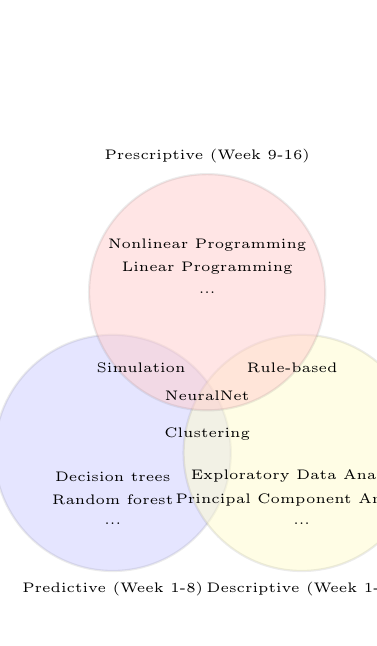
\begin{tikzpicture}[scale=0.6, font=\tiny]
	\useasboundingbox (2.2, -3.5) rectangle (9, 9);
	% Define styles
	\tikzstyle{pred}=[circle, thick, draw=black!75, fill=blue!20, minimum size=30mm, align=center, label=below:, draw opacity=0.1, fill opacity=0.5]
	\tikzstyle{pres}=[circle, thick, draw=black!75, fill=red!20, minimum size=30mm, align=center, label=below:, draw opacity=0.1, fill opacity=0.5]
	\tikzstyle{desc}=[circle, thick, draw=black!75, fill=yellow!20, minimum size=30mm, align=center, label=below:, draw opacity=0.1, fill opacity=0.5]

 	\node[pred, label=below:Predictive (Week 1-8)] (A) at (4,0) {};	
  	\node[desc, label=below:Descriptive (Week 1-8)] (C) at (8,0) {};
	\node[pres, label=above:Prescriptive (Week 9-16)] (B) at (6,3.4) {};

	 %\node at (4,0) {Predictive Analytics (Part 1)};
		 \node at (4,-0.5) {Decision trees};
		 \node at (4,-1) {Random forest};
		 \node at (4,-1.5) {...};
	 %\node at (6,3.4) {Prescriptive Analytics (Part 2)};
		 \node at (6,3.9) {Linear Programming};
		 \node at (6,4.4) {Nonlinear Programming};
		 \node at (6,3.4) {...};
     %\node at (8,0) {Descriptive Analytics (Part 1)};
		 \node at (8,-0.5) {Exploratory Data Analysis};
		 \node at (8,-1) {Principal Component Analysis};
		 \node at (8,-1.5) {...};

	 \node at (6,1.2) {NeuralNet};
	 \node at (7.8,1.8) {Rule-based};
	 \node at (4.6,1.8) {Simulation};
	 \node at (6,0.4) {Clustering};
\end{tikzpicture}        
    \end{figure}    
\end{frame}


\begin{frame}{Topics Covered in Part 2}
    \begin{enumerate}[<+->]
        \item Overview of Prescriptive Analytics Projects
        \item Optimization Modeling Basics
        \item Data-Driven Optimization
        \item Verification and Validation (V\&V)
        \item Optimization Solvers
        \item Evaluation and Benchmarking
        \item Monitoring and Maintenance
        \item Beyond This Course
    \end{enumerate}    
\end{frame}


\begin{frame}{Available Resources}
    \begin{itemize}[<.->]
        \item \textbf{Course website}: \url{https://analytics-project-simt-its.github.io/}
        \item \textbf{Lectures and presentations} (every Friday, 6:30-8:10 PM, on Zoom)
        \item \textbf{Reading materials} (posted in MyITS classroom every week)
        \item  \textbf{Lecture recordings and slides} (in MyITS and the course website)
        \item \textbf{Office hours} (every Saturday, 8-9 AM, on Zoom)
    \end{itemize}    
\end{frame}


\begin{frame}{Assignments}
    \begin{itemize}[<+->]
        \item Due dates \& weights also listed in the course website:        
        \begin{enumerate}[<+->]
            \item Reflection 1 \& 2 (10\%), due Nov 1 \& Dec 13
            \item Proposal presentation (10\%), due Nov 8, 15, \& 22 (random order)
            \item Midterm report (15\%), due Nov 15
            \item Peer review (10\%), due Nov 22        
            \item Final report (25\%), due Dec 13
            \item Final presentation (30\%), due Dec 13
            \item Project repo/website (extra 5\%), due Dec 13
        \end{enumerate}
        \item Rubrics (strict) are available in the course website
        \item Deadlines are 23:59:59 AoE (Anywhere on Earth)
    \end{itemize}
\end{frame}


\begin{frame}{Course Schedule (screenshot of the course website)}
    \begin{figure}
        \centering
        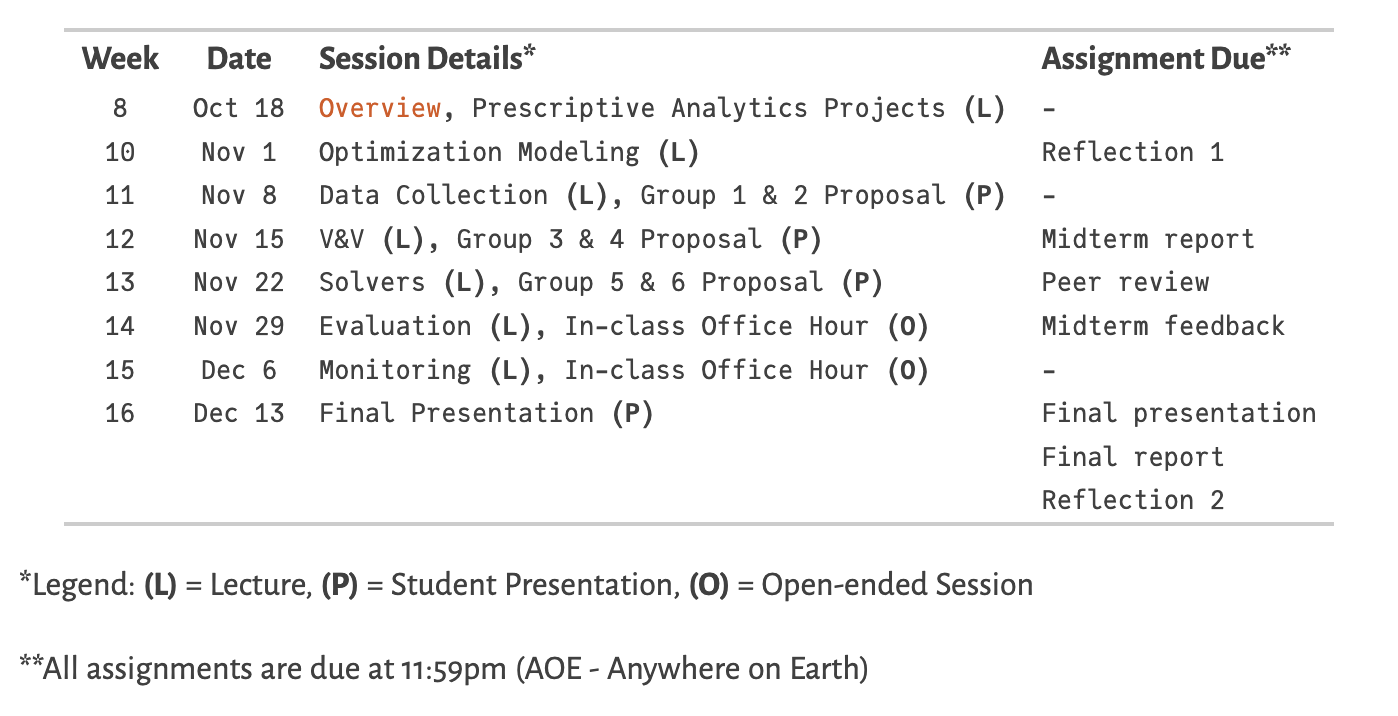
\includegraphics[width=0.9\linewidth]{../fig/schedule.png}        
    \end{figure}  
\end{frame}

\begin{frame}{AI Usage Policy}
    \begin{itemize}[<+->]
        \item \textbf{You may use AI tools} and libraries for your projects.
        \item However, you must use them \textbf{ethically} and \textbf{responsibly}.
        \item Any AI-assisted work must be \textbf{clearly stated} in your reports and presentations.
        \item For any AI-assisted assignments, you must also \textbf{submit AI Usage and Reflection Form}: \url{https://mansurarief.github.io/ai-usage-and-reflection-form.docx}
        \item See the course website for the \textbf{full policy}.
    \end{itemize}
\end{frame}

\begin{frame}{Take Care of Yourself}
    \begin{itemize}[<+->]
        \item \textbf{Mental health} is important. If you feel overwhelmed with the course, please reach out to me. \textbf{I am here to help.}
        \item \textbf{Physical health} is also important. Please get enough sleep. It is okay to ask for extension if you are not feeling well.
        \item \textbf{Time management} is crucial. Do not wait until the last minute to work on your assignments (especially the final project).
        \item \textbf{Academic integrity} is a must. This class has absolutely 0 tolerance for cheating. You will fail this class if you do not do your own work.
    \end{itemize}
\end{frame}

\begin{frame}{How to Reach Me}
    \begin{itemize}[<+->]
        \item \textbf{Email} is your best bet: 
        \begin{itemize}
            \item \url{mansur.maturidi@its.ac.id}, 
            \item + cc \url{mansur.arief@stanford.edu} (if you want more visibility)
        \end{itemize}
        \item \textbf{Office hours} every Saturday, 8-9 AM, on Zoom. The link will be posted in MyITS.
        \item \textbf{By appointment}: if you cannot make it to the office hours but need to talk to me, set up an appointment at \url{https://mansurarief.github.io/calendar/}
        \item \textbf{WhatsApp}: If you think it is urgent, send me a WA message at +1-734-881-0531 (though note that we live in different time zones).
    \end{itemize}
\end{frame}

\begin{frame}{Ask me questions about the course!}
    \begin{itemize}[<.->]
        \item Let's take a few minutes break to ask questions about the course.
    \end{itemize}
\end{frame}
    
\section{Introduction}
\begin{frame}{Your turn}
    \begin{itemize}[<.->]
        \item Please introduce yourself (30 sec - 1 min each):
        \begin{itemize}
            \item Name, year of study, \& current position and institution
            \item How much (hands on) experience do you have in optimization or data processing?
        \end{itemize}
    \end{itemize}
\end{frame}

\section{Prescriptive Analytics Projects}

\begin{frame}{Prescriptive Analytics Scope}
    \begin{itemize}[<.->]
        \item \textbf{Descriptive analytics}: analyzing what has happened in the past
        \item \textbf{Predictive analytics}: predicting what is likely to happen in the future.
        \item \textbf{Prescriptive analytics}: using data to \emph{recommend actions} that will \emph{optimize outcomes}.
    \end{itemize}
\end{frame}

\begin{frame}{[Exercise 1.1] Scope of each analytics type}

    \begin{enumerate}[<.->]
        \item List of products sold last year and their sales volume aggregated by month and by stores 
		\item Statistical summary of sales data (average, standard deviation, and trends) for each product
		\item Clustering of products based on sales volume and their co-occurrences
		\item Forecast of sales for the product clusters for the next quarter
		\item Simulation and what-if analysis of different promotion strategies
		\item Recommendations for pricing strategies to increase sales
		\item Allocation of marketing budget across different product categories
    \end{enumerate}

  
    Which of the above items belong to \textbf{descriptive, predictive, and prescriptive analytics?}

\end{frame}

\begin{frame}{Major Steps in Prescriptive Analytics Projects}

    \begin{enumerate}[<+->]
        \item Problem scoping and definition
        \begin{itemize}[<.->]
            \item Define the objectives and tdentify stakeholders and their needs
        \end{itemize}
        \item Data collection
        \begin{itemize}[<.->]
            \item Identify data sources
            \item Collect and preprocess data
            \item Data quality assessment
            \item Data privacy and security
            \item Data storage and management
            \item Data visualization
        \end{itemize}
        \item Optimization process 
        \item Implementation and monitoring
    \end{enumerate}
\end{frame}

\begin{frame}{Problem Scoping and Definition}
    \begin{itemize}[<+->]
        \item What are the business objectives of the project?
        \item What are the key performance indicators (KPIs) that will measure the success of the project?
        \item Who are the stakeholders involved in the project, and what are their roles and responsibilities?
        \item What data sources are available? How much can we trust the data? Are there any limitations or biases in the data that we need to be aware of?
        \item What are the expected outcomes of the project, and how will the results be used to make decisions?
    \end{itemize}
\end{frame}

\begin{frame}{[Exercise 1.2] Discuss with your group}
    You are a sales manager tasked to increase sales for the upcoming quarter. You want to optimize allocation of the marketing budget to achieve this goal. You work with the marketing team, the sales team, the inventory management team, and the data and IT for the project.
    
    \begin{enumerate}
        \item The marketing team has historical data on the marketing budget allocation for all products, but they only use customer engagement metrics.
        \item The sales team has data on the sales volume for each product item but only record sales if the product is in stock.
        \item The inventory team has data on the inventory levels for each product item and the order received from the sales team, but not on lost sales.
        \item The data and IT team maintains the data infrastructure and systems for the company. They can provide historical data and predictive models for sales volume with 100\% accuracy!
    \end{enumerate}
    
    \textbf{Identify a proper scope for the project! What risks and obstacles you might face?}
\end{frame}

\begin{frame}{What's next?}
    \begin{itemize}[<+->]
        \item Next week: 
        \begin{itemize}[<+->]
            \item Discuss the group acvitity (Exercise 1.2)
            \item Optimization Modeling Basics
        \end{itemize}
        \item Next reading: Ch. 2 -- Optimization Modeling
        \item Upcoming assignment: Reflection 1 (due Nov 1)
        \item No office hour for Oct 19.
    \end{itemize}
\end{frame}

\begin{frame}{Thank you!}
    \begin{itemize}[<+->]
        \item Questions?
    \end{itemize}
\end{frame}











\end{document}
